\chapter*{Risikomanagement}
	\documentPartEntry{Risikomanagement}
	
	\label{risiken}
	
	\section*{Übersicht über die Risiken}
		Um die Risiken im Projekt zu kennen und Massnahmen zu deren Minimierung umsetzen zu können, haben wir zu Beginn des Projekts eine Risikoanalyse erstellt und diese während des Projektverlaufs nach dem Abschluss jedes Meilensteins überarbeitet.
		In Abbildung~\ref{fig:RiskMatrix} und \ref{fig:RiskMatrixWeightedDamage} sind die im Kapitel~\ref{einzelneRisiken} detailliert aufgeführten Risiken in einer Übersicht dargestellt.
		
		\begin{figure}[H]
			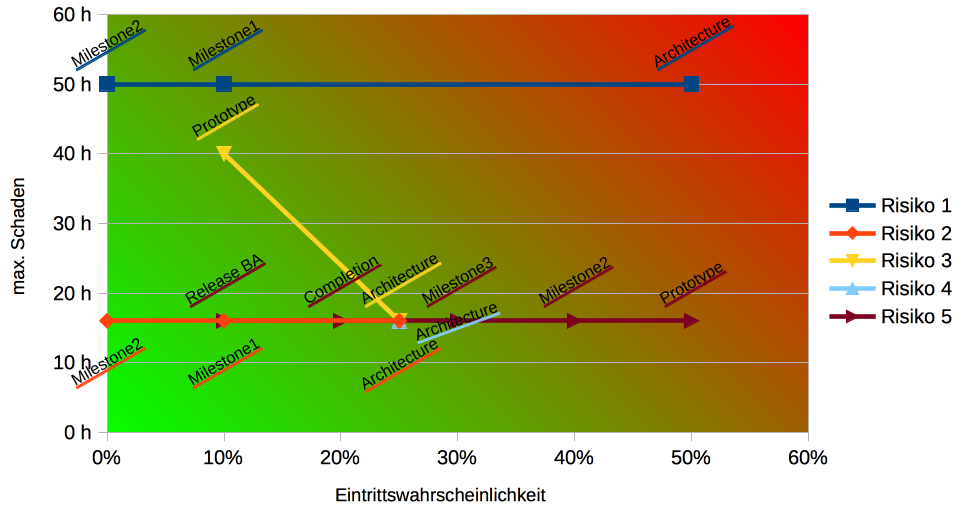
\includegraphics[width=0.9\textwidth]{projectPlan/media/img/risikomatrix.png}
			\centering
			\caption{Risikomatrix}
			\label{fig:RiskMatrix}
		\end{figure}
	
		Abbildung~\ref{fig:RiskMatrix} zeigt übersichtlich in Form eines X/Y-Diagramms welches Risiko wie wahrscheinlich ist (X-Achse) und wie gross der Schaden maximal bei einem Eintritt geschätzt wurde (Y-Achse).
		Dabei sind jeweils für jedes Risiko die geschätzten Werte bei den Milestones eingetragen.
		
		Es ist deutlich zu sehen, dass das Risiko~1 dabei zu Beginn am kritischsten war und deshalb möglichst früh angegangen wurde.
		Natürlich haben wir auch für die übrigen Risiken Massnahmen getroffen.
		Die für jedes Risiko getroffenen vorbeugenden Massnahmen sind im Kapitel~\ref{einzelneRisiken} direkt bei jedem Risiko selbst aufgeführt.
	

	\section*{Einzelne Risiken}\label{einzelneRisiken}
		\newcounter{riskidcounter}
		
		\newcommand{\riskTable}[3]{
			%Die Spalten werden aufgeteilt auf dem goldenen Schnitt
			\noindent
			\refstepcounter{riskidcounter}
			\begin{tabular}{|p{\smallThird\textwidth} | p{\largeThird\textwidth} |}
				\hline	
				Risiko-ID 		& Risiko \theriskidcounter \\
				\hline
				Titel 			& #1 \\
				Beschreibung 		& #2 \\
				Bewertung		&
				\begin{minipage}[b]{\linewidth}
					\begin{figure}[H]
						\includegraphics[width=0.9\textwidth]{projectPlan/media/img/risiko\theriskidcounter.png}
						\centering
						\caption{Bewertung Risiko \theriskidcounter}
						\label{fig:Risk\theriskidcounter}
					\end{figure}
				\end{minipage} \\
				Vorbeugung/Massnahmen		& #3 \\
				\hline
			\end{tabular}
			\hspace{0.5cm}
			\newline	
		}
		
		\riskTable{Qualität der DKS Schnittstelle}
		{Die Schnittstelle entspricht nicht den Anforderungen des Projektes und liefert zu wenige Informationen.}
		{Eignung der Schnittstelle durch den Prototyp abklären.}
		
		\riskTable{Einarbeitung Play Framework}
		{Die Einarbeitung des Teammitglieds, welches das Play Framework noch nicht kennt, dauert länger als angenommen.}
		{Rechtzeitiges Einarbeiten ins Framework}
		
		\riskTable{Mapping Complexity}
		{Die Abbildung des Metamappings ist wesentlich komplexer als angenommen.}
		{Minimales Mapping bereits im Prototyp umsetzen um Komplexität abschätzen zu können. Mapping Features priorisieren, die Kernfunktionalität abdecken, Nebenfunktionalität weglassen.}

		\riskTable{Schnittstelleneinheitlichkeit}
		{Die Schnittstellen der gängigen Projektmanagementsysteme sind zu unterschiedlich, als das sie über einen Adapter mit einer Konfiguration abgedeckt werden können.}
		{Bereits während der Prototypenphase verschiedene Schnittstellen berücksichtigen.}

		\riskTable{Ausfall Infrastruktur}
		{Die Infrastruktur des Projekts fällt aus.}
		{Regelmässig Backups der kritischen Daten erstellen.}
